\chapter{Used Technologies}\label{sec:technologies}
In this chapter technologies that were used during development will be described.
Also the motivation for the usage of these technologies will be explained.

\section{Platform}
In the following section technologies that were used to build a cloud platform will be described.
These technologies have made it possible to build a scalable solution with an easy deployment.

Traditionally, a deployment of a such a complex system as CloudASR consists of several steps
  during which necessary dependencies are installed,
  the application environment is set up
  and finally the application is started.
But this approach makes the maintenance of these systems difficult,
  because the deployment is time consuming, error-prone and it is not replicable.
The ultimate goal for the CloudASR deployment was the exact opposite: fast and replicable deployment.

The most important tool used during the development was \textbf{Docker} \cite{merkel2014docker}
  -- a portable, lightweight application runtime and packaging tool.
It allows to specify dependencies and environmental variables for a process
  and it allows to build an image from this specification called Dockerfile
  (see Figure~\ref{fig:dockerfile} for example).
Once this image is built it can be used on any machine with Docker installed,
  which makes the deployment fast and replicable,
  because it is not necessary to install all dependencies on every machine.
Additionally, the usage of Docker images removes bugs caused by different versions of libraries used in development and production environment
  because developers use the same images in both environments.

\begin{figure}[h]
  \verbatiminput{snippets/Dockerfile}

  \caption{
    An example of Dockerfile that creates an image from the base Ubuntu image,
      installs python,
      copies all files in the Dockerfile folder
      and sets command python run.py to be run,
        when the docker image is started.
  }
  \label{fig:dockerfile}
\end{figure}


When running an application in the cloud it is neccessary to monitor all servers and handle failovers.
But with an increasing number of servers, maintenance costs grow rapidly.
Therefore, it is not possible to manage the application manually.
The tool that allows CloudASR to run on many servers is \textbf{Mesos} \cite{hindman2011mesos}.
It lets users program against a set of machines in the same way as if it was a single machine,
  which means that it is possible to run and scale an application on a set of servers in a similar way as on a single machine.
Mesos takes care of the scheduling and high availability of the platform.
Thus, whenever some part of the CloudASR crashes, Mesos will try to restart it.
Finally, Mesos supports Docker so the images that are used in development can be also used on a Mesos cluster.

\textbf{Marathon}\footnote{\url{https://mesosphere.github.io/marathon/}} is a framework built on top of Mesos whose main responsibility is to launch long running applications.
It is an entrypoint for running and scaling the applications running on a Mesos cluster.
It has a web user interface (see Figure~\ref{fig:marathon}) and a REST API,
  through which applications can be started, scaled or stopped easily.

\begin{figure}
  \centering
  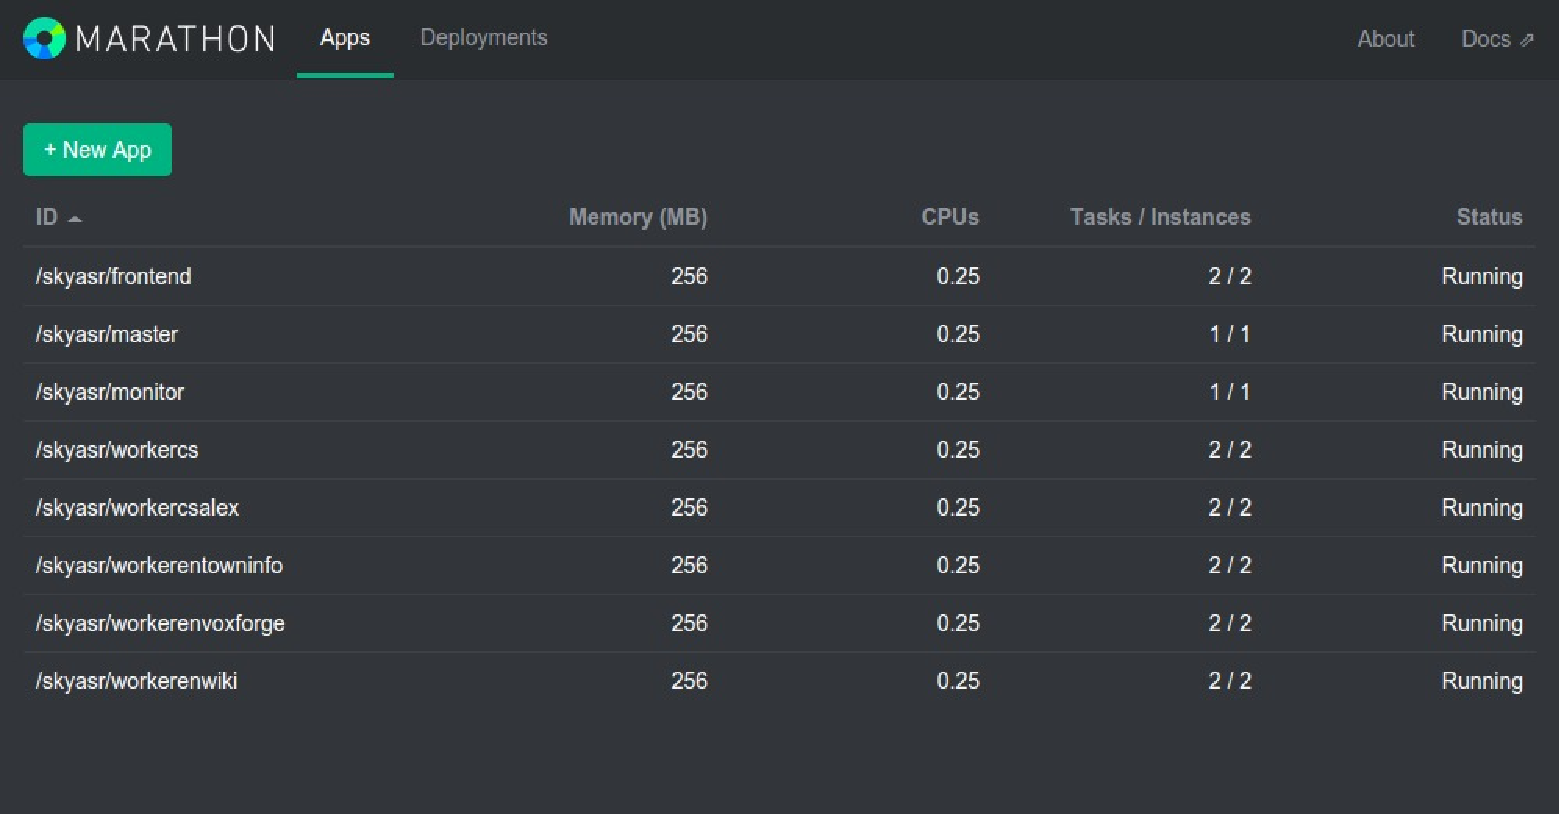
\includegraphics[width=0.95\textwidth]{./img/marathon.pdf}

  \caption{
    A screenshot of a Marathon web interface with a running CloudASR platform.
  }
  \label{fig:marathon}
\end{figure}

Since the traffic of CloudASR platform can be very large,
  it is not possible to process all HTTP requests by one application server.
Therefore, CloudASR platform uses \textbf{HAProxy}\footnote{\url{http://www.haproxy.org/}} load-balancer to distribute workload between application servers,
  but any other load-balancers can also be used with appropriate setup.



\section{Continuous Integration \& Delivery}
Several practises were obeyed during the development,
  namely Continuous Integration and Continuous Delivery.
For this a platform which consisted of \textbf{Jenkins-CI}\footnote{\url{https://jenkins-ci.org/}} and \textbf{Docker Registry}\footnote{\url{https://github.com/docker/docker-registry}} was deployed.

The most important tool for Continuous Integration \& Delivery of CloudASR is Jenkins-CI.
Its task is to watch CloudASR git repository
  and whenever a new code is pushed into this repository it schedules a new build of the platform.
During this build, the most recent code is pulled from the repository and then the new docker images are built.
After that tests are run to check that the new code did not break anything.
Finally, successfully built images are tagged with current build number and pushed to the Docker Registry.


Docker Registry is a repository of Docker images.
Even though, there are several Docker Registry providers\footnote{\url{https://hub.docker.com/}, \url{https://quay.io/}},
  which are free for open-source projects,
  CloudASR uses its own free Docker Registry in order to be able to use also proprietary software that cannot be shared with public.


\section{Backend}
The main programming language used for backend development is \textbf{Python}\footnote{\url{https://www.python.org/}}.
The web interface is built on top of \textbf{Flask}\footnote{\url{http://flask.pocoo.org/}} microframework
  and it uses \textbf{Gunicorn}\footnote{\url{http://gunicorn.org/}} for production deployment.
\textbf{MySQL}\footnote{\url{https://www.mysql.com/}} is used as a database,
  but any other SQL database can be used instead,
  because the database is accessed  through \textbf{SQLAlchemy}\footnote{\url{http://www.sqlalchemy.org/}}.

The CloudASR architecture consists of several nodes which need to communicate between each other.
CloudASR uses \textbf{ZeroMQ}\footnote{\url{http://zeromq.org/}} for this communication
  because of its simple design, high performance and support for every modern language.
With ZeroMQ,
  it is possible to create many messaging patterns,
  but CloudASR uses only two: request-reply and push-pull.
In the request-reply messaging pattern a sender sends a message and then waits for a reply,
  after that another sender can send next message and wait for a reply.
On the other hand, in the push-pull messaging pattern senders just send messages and do not wait for replies.


In order to be able to send complex messages via ZeroMQ sockets, messages have to be serialized.
CloudASR uses \textbf{Google Protocol Buffers}\footnote{\url{https://developers.google.com/protocol-buffers/}},
  because they have support in many languages,
  allow specification of various message types (See Figure~\ref{fig:protobuf} for example)
  and serialize messages in very compact way
  (See Table~\ref{fig:protobuf-benchmark} for a comparison of different serializations).

\begin{figure}[h]
  \verbatiminput{snippets/protobuf.proto}

  \caption{
    An example of Google Protocol Buffer message specification with three fields.
    Fields address and model are just strings and the status is an enum with four possible values.
  }
  \label{fig:protobuf}
\end{figure}

\begin{table}[h]
  \begin{tabular}{rrl}
  \textbf{raw file size} & 56146 & \\
  \cline{1-3}
  \textbf{bytes\_protobuf} & 56118 & 0.999x \\
  \textbf{base64} & 74872 & 1.333x \\
  \textbf{json\_array} & 158590 & 2.824x \\
  \end{tabular}

  \caption{
    The table shows comparison of different serialization used to serialize a wave file into a message for the CloudASR online mode.
    As can be seen from the results Google Protocol Buffers achieved the best result.
  }
  \label{fig:protobuf-benchmark}
\end{table}

CloudASR uses \textbf{Pykaldi} \cite{platek2014free} as a Python wrapper for the \textbf{Kaldi speech recognition toolkit} \cite{povey2011kaldi}.
Because CloudASR should be able to process very long recordings, possibly infinite,
  with limited computational resources,
  it is necessary to split the recordings into smaller chunks.
For that purpose CloudASR uses voice activity detector implemented in \textbf{Theano} \cite{bergstra2010theano} to detect silences in a speech.


\section{Frontend}
The frontend uses several well-known open-source libraries, namely,
  \textbf{Twitter Bootstrap}\footnote{\url{http://getbootstrap.com/2.3.2/}} for CSS styling of the web,
  \textbf{jQuery}\footnote{\url{https://jquery.com/}}
  and \textbf{Angular.js}\footnote{\url{https://angularjs.org/}} for interactive elements on the web.

\begin{figure}[h]
  \centering
  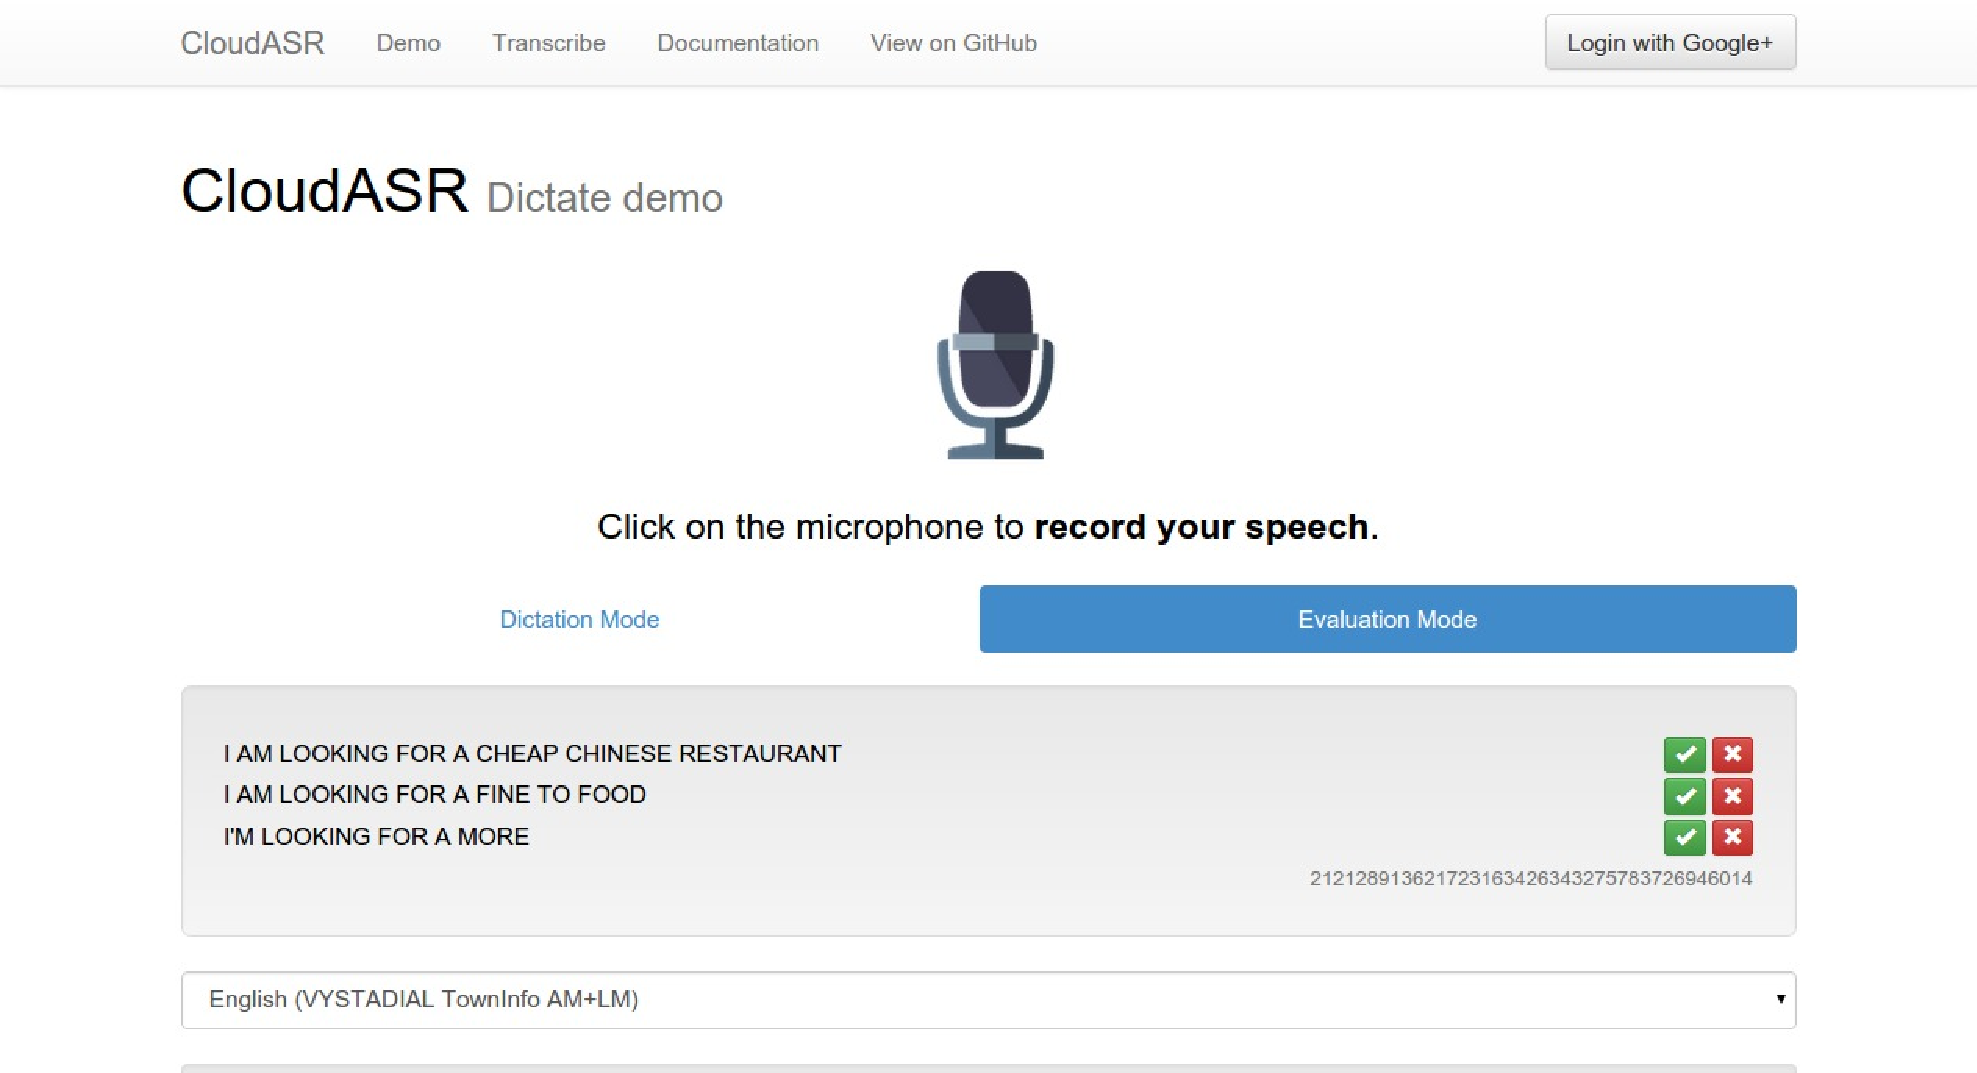
\includegraphics[width=0.95\textwidth]{./img/demo.pdf}

  \caption{Screen of the Web Demo}
  \label{fig:demo}
\end{figure}

Modern web browsers support \textbf{WebAudio API}\footnote{\url{http://webaudio.github.io/web-audio-api/}},
  which is a high-level JavaScript API for processing and synthesizing audio in web applications.
One of the things that can be done with this API is audio recording.
Thus, it is possible to create a web demo for the CloudASR online mode.
The demo is based on \textbf{Recorder.js}\footnote{\url{https://github.com/mattdiamond/Recorderjs}} library,
  which can record output of WebAudio API and return it as a PCM chunks.

The next step is to send these chunks to the API.
Because the demo demonstrates the online speech recognition mode,
  it is not possible to wait for the whole recording to be recorded and then send it to the API via HTTP POST request.
Thus, CloudASR uses \textbf{Socket.IO}\footnote{\url{http://socket.io/}} to send stream of chunks to the API
  and to receive stream of results from the API.
